\documentclass[border=6pt]{standalone}
\usepackage{fontspec,xeCJK,amsmath,amssymb,tikz,graphicx}
\usetikzlibrary{arrows.meta}
\setmainfont{Arial}\setCJKmainfont{PingFang SC}
\definecolor{ink}{HTML}{203340}\definecolor{blue}{HTML}{147E91}\definecolor{pale}{HTML}{EFF6F5}\definecolor{line}{HTML}{D3E0DF}\definecolor{warm}{HTML}{BA652C}
\begin{document}\begin{tikzpicture}[x=1cm,y=1cm,every node/.style={text=ink,font=\fontsize{10}{13}\selectfont},flow/.style={-{Stealth[length=5pt]},draw=blue,line width=1pt}]
\path[use as bounding box](0,0)rectangle(11,29.2);\fill[pale](0,0)rectangle(11,29.2);
\node[font=\fontsize{19}{23}\selectfont\bfseries]at(5.5,28.4){3DGS：把场景画成可优化的椭球};
\node[text=blue]at(5.5,27.7){固定场景多视角重建 · 新视角实时渲染};
\draw[rounded corners=6pt,draw=line,fill=white](.35,22.2)rectangle(10.65,27.0);
\node[anchor=west,font=\fontsize{13}{16}\selectfont\bfseries]at(.65,26.45){A　输入与初始化};
\node at(2.15,24.3){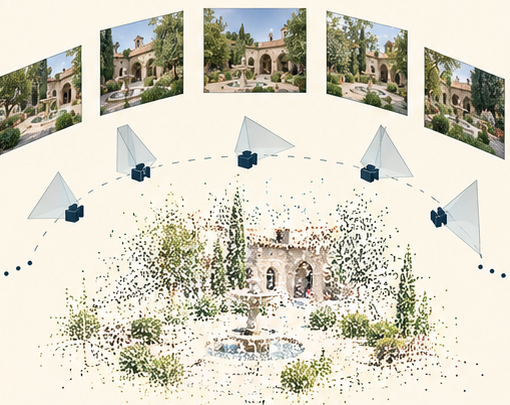
\includegraphics[width=2.8cm,height=2.7cm,keepaspectratio]{visual-1.png}};
\node[anchor=west]at(3.8,25.5){多视角 RGB + SfM 相机位姿};
\node[anchor=west]at(3.8,24.78){稀疏点初始化高斯中心 $\mu\in\mathbb R^3$};
\node[anchor=west]at(3.8,24.06){初始尺度/旋转/不透明度/颜色};
\node[anchor=west]at(3.8,23.34){对应正文 §2--3；不先求完整网格};
\draw[flow,dotted](5.5,22.2)--(5.5,21.8);
\draw[rounded corners=6pt,draw=line,fill=white](.35,17.0)rectangle(10.65,21.8);
\node[anchor=west,font=\fontsize{13}{16}\selectfont\bfseries]at(.65,21.25){B　空间高斯};
\node at(2.15,19.1){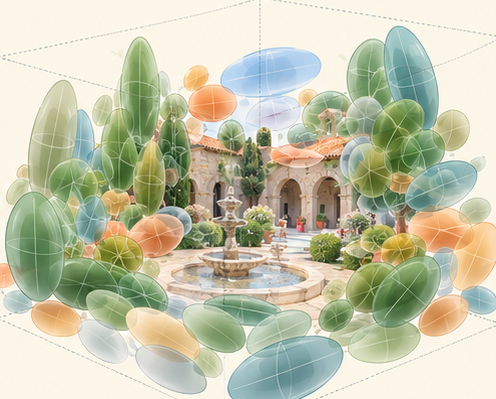
\includegraphics[width=2.8cm,height=2.7cm,keepaspectratio]{visual-2.png}};
\node[anchor=west]at(3.8,20.3){尺度3维；旋转单位四元数4维};
\node[anchor=west]at(3.8,19.580000000000002){协方差 $\Sigma=RSS^TR^T\in\mathbb R^{3\times3}$};
\node[anchor=west]at(3.8,18.86){不透明度 $o$；球谐表达视角相关颜色};
\node[anchor=west]at(3.8,18.14){对应正文 §4；数量可随训练改变};
\draw[flow,dotted](5.5,17.0)--(5.5,16.6);
\draw[rounded corners=6pt,draw=line,fill=white](.35,11.8)rectangle(10.65,16.6);
\node[anchor=west,font=\fontsize{13}{16}\selectfont\bfseries]at(.65,16.05){C　投影与合成};
\node at(2.15,13.900000000000002){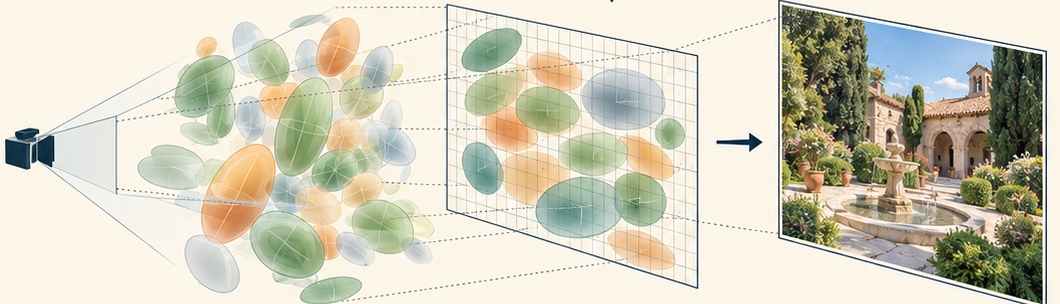
\includegraphics[width=2.8cm,height=2.7cm,keepaspectratio]{visual-3.png}};
\node[anchor=west]at(3.8,15.100000000000001){局部投影：三维协方差 $\to$ 二维椭圆};
\node[anchor=west]at(3.8,14.38){16$\times$16 tile；复制/排序可见高斯};
\node[anchor=west]at(3.8,13.660000000000002){由近到远 alpha 合成；遮挡累积};
\node[anchor=west]at(3.8,12.940000000000001){对应正文 §4、§6；训练与查看共用};
\draw[flow,dotted](5.5,11.8)--(5.5,11.4);
\draw[rounded corners=6pt,draw=line,fill=white](.35,6.599999999999999)rectangle(10.65,11.399999999999999);
\node[anchor=west,font=\fontsize{13}{16}\selectfont\bfseries]at(.65,10.849999999999998){D　优化与密度控制};
\node at(2.15,8.7){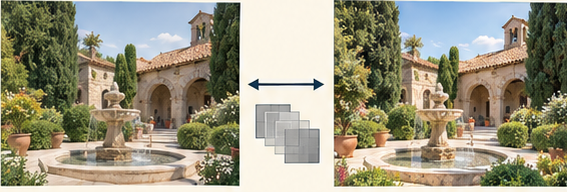
\includegraphics[width=2.8cm,height=2.7cm,keepaspectratio]{visual-4.png}};
\node[anchor=west]at(3.8,9.899999999999999){渲染图对照真值：0.8 L1 + 0.2 D-SSIM};
\node[anchor=west]at(3.8,9.179999999999998){反传更新位置/尺度/旋转/颜色/不透明度};
\node[anchor=west]at(3.8,8.459999999999999){小且欠覆盖：clone；大且欠细节：split};
\node[anchor=west]at(3.8,7.739999999999998){低不透明度 prune；对应正文 §5};
\draw[flow,dotted](5.5,6.599999999999999)--(5.5,6.199999999999998);
\draw[rounded corners=6pt,draw=line,fill=white](.35,1.3999999999999995)rectangle(10.65,6.199999999999999);
\node[anchor=west,font=\fontsize{13}{16}\selectfont\bfseries]at(.65,5.6499999999999995){E　新视角与检验};
\node at(2.15,3.499999999999999){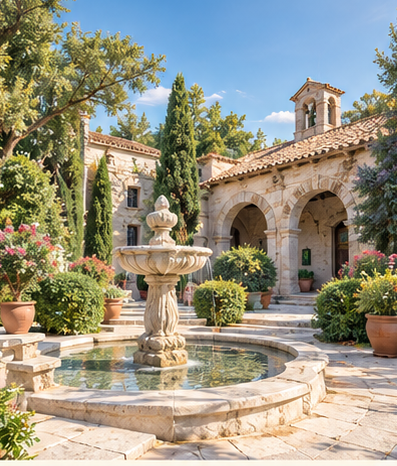
\includegraphics[width=2.8cm,height=2.7cm,keepaspectratio]{visual-5.png}};
\node[anchor=west]at(3.8,4.699999999999999){固定已训练高斯，换相机 $\to$ C $\to$ 图像};
\node[anchor=west]at(3.8,3.9799999999999995){Table 1：质量 / FPS / 时间 / 存储};
\node[anchor=west]at(3.8,3.2599999999999993){Table 3：初始化、拆分、形状与颜色消融};
\node[anchor=west]at(3.8,2.539999999999999){对应正文 §7--8；静态外观表示};
\end{tikzpicture}\end{document}